\documentclass{article}


\usepackage{hyperref}
\usepackage{soul}
\usepackage{tabularray}
\usepackage{listings}
\usepackage{amsmath}
\usepackage{amssymb}
\usepackage{fancyhdr}
\usepackage{geometry}
\usepackage[swedish]{babel}
\usepackage{graphicx}

\setlocalecaption{swedish}{table}{Tabell }
\setlocalecaption{swedish}{contents}{Innehåll}
\geometry{a4paper}
\geometry{left=45mm,right=45mm,bottom=20mm,top=20mm}

\setlength{\parskip}{\baselineskip}
\setlength{\parindent}{0cm}

\title{Chlang - ${94^{404}}$\hspace*{0.2cm} schackbotar}
\author{Tage Danielsson}
\date{\parbox{\linewidth}{\centering%

\includegraphics{./images/white-king.png}\endgraf
E-Mail: danielsson.dev@gmail.com\endgraf
Skola: Hitachigymnasiet Västerås\endgraf
Kurs: Gymnasiearbete \endgraf
Läsår: 2024-2025\endgraf
}}

\fancypagestyle{plain}{%
    \fancyhf{}
    \fancyfoot[C]{\thepage}
    \renewcommand{\headrulewidth}{0cm}
    \renewcommand{\footrulewidth}{0.01cm}
}

\pagestyle{plain}

\begin{document}
	\selectlanguage{swedish}
	\pagenumbering{gobble}
	\maketitle
	\thispagestyle{empty}
	\tableofcontents
	\newpage
	\pagenumbering{arabic}

	\section{Sammanfattning}
	Chlang är ett språk som är anpassat för att skapa evalueringsfunktioner som tillsammans med en trädsökningsalgoritm bildar en schack-bot. En fil med innehållande chlang kan kompileras med hjälp av chlang kompilatorn för att skapa en sträng med 404 stycken specifika (mellan ascii värde 33 och 126) ascii tecken som sedan kan laddas in i något av chlang interfacen (webbsidan är lättast att använda), man kan då spela mot boten som representeras av strängen. Tanken med språket, som representeras av vilken (i princip) ascii sträng som helst med längden 404, är att man enkelt ska kunna dela botar (då strängen kan fungera som ett bott id), generera botar med algoritmer (då detta är lika enkelt som att skriva en algoritm som genererar strängen) och skapa botar från berättelser (här finns ju tyvärr begränsningen av att till exempel å,ä och ö inte kan användas och att längden måste vara exakt 404, även mellanslag är otillåtet så man får i dessa fall använda till exempel understreck). Tanken är också att man ska kunna träna botar med en genetisk algoritm, men detta går för tillfället långsamt och har inte gett några bra resultat. Man ska också kunna ta en sträng och köra kompilatorn baklänges för att få chlang igen men detta ingår fortfarande i sectionen vidare utveckling.

	Chlang programmen och platformarna har utvecklats under läsåret 2024-2025. Samtliga är skrivna i programmeringspråket rust, men web-applikationen har även en html-fil. Flera verktyg, bibliotek och ramverk har använts under utvecklandet, dessa är:
	\begin{description}
	\item [Hyperfine] - för prestandamätning
	\item [Cargo Flamegraph] - för prestandamätning och visualisering
	\item [Rand] - ett rust bibliotek för slumptalsgenerering.
	\item [Rustc-hash] - ett rust bibliotek för snabbare hashfunktioner
	\item [Backtrace-on-stack-overflow] - ett rust bibliotek för felsökning
	\item [Leptos] - ett web ramverk för rust/wasm (för web applikation)
	\item [Gloo-timers] - ett rust bibliotek för att hantera timers (som futures) i wasm.
	\item [Pix-engine] - en spel-motor för rust (för native gui)
    \item [Trunk] - ett cli-verktyg för att bygga och testa webapplikationer skrivna i rust.
	\end{description}
	  
	
	\section{Abstract}
	Chlang is a language created for the configuration of custom evaluation functions that, together with a tree search, makes for a chess bot. A file containing valid chlang can be compiled using the chlang compiler to create a 404-character long string containing ascii characters between the values 33 and 126. These can then be loaded by one of the chlang runtimes (The website is the most accessible one) after wich you can play the chess bot represented by the string. The idea is that it should be easy to share bots (since the string is essentially an id), generate bots using code (since it's as easy as generating a string) and create bots from stories (this is a little limited since characters from other languages, such as the swedish "åäö" can not be used and space is also prohibited and has to be substituted with for ex (since it's as easy as generating a string) and create bots from stories (this is a little limited since characters from other languages, such as the swedish "åäö", can not be used and space is also prohibited and has to be substituted with for example an underscore). In theory it should also make it easy to train bots using a genetic algorithm but in practice this have been slow and have not produced any good results. You are also supposed to be able to decompile the string into chlang so that you can easily analyze generated/trained bots. This is still in the chapter "Vidare Utveckling" (Further Improvements).

	The chlang programs and platform are all writen in the programming language rust during the academic year of 2024-2025. The web version also includes a single html file. A couple of tools, libraries and frameworks were used during the development, these are:
	\begin{description}
	\item [Hyperfine] - for benchmarks
	\item [Cargo Flamegraph] - for benchmarks, cpu-profiling and visualisation
	\item [Rand] - a rust library for random number generation
	\item [Rustc-hash] - a rust library for faster hashing functions
	\item [Backtrace-on-stack-overflow] - a rust library for debugging
	\item [Leptos] - a web framework for rust/wasm (used for web interface)
	\item [Gloo-timers] - a rust library for handling timers and futures in wasm.
	\item [Pix-engine] - a game engine for rust (used for windows gui)
    \item [Trunk] - a cli-tool for building and testing rust-wasm webapplications.
	\end{description}
	
	\section{Inledning}

	\subsection{Syfte}
	Syftet med chlang är att skapa intresse för skapandet av schackbotar genom att göra det roligt, lättillgängligt och enkelt att dela.
	
	\subsection{Bakgrund}
	Det finns såklart redan andra schackbotar, det som gör chlang unikt är att så många olika strängar representerar en giltig schackbot. Det skapar möjligheter för att dela botar, generera botar, testa botar och leka med tanken av att skapa botar som representeras av till exempel namn, text och/eller skämt.
	
	\subsection{Frågeställning}
	Går det att representera en schackbot med vilken sträng som helst och hur skulle dessa botars beteenden variera?

	\newpage
	\section{Teori}
    Det krävs inte någon särskilt teknisk förkunskap för att läsa denna
    rapport men grundläggande kunskaper om schackbegrepp/schackregler såsom
    "En-Passant" eller "50-dragsregeln" kan göra det enklare att hänga med. 
    Den tekniska kunskapen som skulle kunna hjälpa läsaren är att förstå vad
    begreppen "struct", "enum" och "trait" innebär i programspråket rust, då
    dessa används i sektionen "Datatyper".
	
	

	\newpage
	\section{Metod}

	\subsection{Delar}	
	För att skapa Chlang så krävdes utveckling av flera olika delar. Därför startades arbetet med planering av vilka delar som skulle ingå och i vilken ordning dessa skulle skapas. Listan har ändrats lite med arbetets gång men ser nu ut såhär:
	\begin{enumerate}
	\item Schackspel:
		\begin{enumerate}
			\item Datastruktur för representering av bräde
			\item Generering av drag
			\item Huvudlöst schackspel (schackspelsapi)
		\end{enumerate}
	\item Schackbotsmotor:
	\begin{enumerate}
	\item Trädsökningsalgoritm
	\item Hårdkodad evalueringsfunktion
	\item Datastruktur och metoder för slutgiltig evalueringsfunktion.
	\item Trädsöksoptimisering (pruning, cache)
	\end{enumerate}
	\item Chlang-språket
	\begin{enumerate}
	\item Konstruktion av evalueringsfunktion från sträng
	\item Kompilator för Chlang
	\item Dekompilator för Chlang (ej färdigt)
	\end{enumerate}
	\item Platformar (interface)
	\begin{enumerate}
	\item Web
	\item Terminal (inte så bra, mest för utveckling)
	\item Gui (inte så bra, mest för utveckling)
	\end{enumerate}
	\item Verktyg
	\begin{enumerate}
	\item Jämför botar
	\item Träna botar
	\end{enumerate}
	\end{enumerate}

	\subsection{Datatyper}
	Programmeringspråket rust har ett mycket kraftfullt datatypssystem som vi utnytjar i chlang. De huvudsakliga beståndsdelarna av chlang är alla representerade som egna datatyper. Dessa inkluderar: 
	\begin{itemize}
	\item Schackbrädet (struct)
	\item Sida [vit/svart] (enum)
	\item Position på brädet (struct)
	\item Typ av pjäs (enum)
	\item Partiets tillstånd (enum)
	\item botar (struct)
	\item Spelare [bot/människa] (enum)
	\item Drag (struct)
	\item Evalueringfunktioner (struct)
	\item Nyckel för bräde (struct)
	\item Flera structs och enums för parsing i kompilatorn
	\end{itemize}	

	\subsection{Verktyg}
	På grund av att prestanda är en så viktig del av schack-botar så blev två verktyg väldigt viktiga. Dessa är Hyperfine och Cargo Flamegraph. Dessutom så kraschade programmet med felmeddelandet "Stack Buffer Overflow" vid en period under arbetet vilket kunde felsökas med hjälp av biblioteket "backtrace-on-stack-overflow".

	Hyperfine användes för att göra prestandamätningar som kunde uttnyttjas för att avgöra om ändringar i projektet ledde till framsteg. En ändring gav en prestandaökning som med hjälp av hyperfine uppmättes till att ge ca 120 gånger högre prestanda.

	Verktyget som förenklade processen av att hitta möjligheten för nämnda prestandaförbättring var "cargo flamegraph". Detta verktyg genererar så kallade "flamegraphs" eller "flamechart" genom att använda linux egna prestandamätare och cpu-profilerare "perf" och sedan sammanställa datan i  en pdf. Genom att kolla på dessa flamecharts upptäcktes möjligheten till prestanda förbättringen då grafen visade att samma frekventa anrop till funktionen "Clone" tog upp en stor del av körningstiden. Förbättringen skedde genom att göra ändringar till koden som tillät utbytet av den kostsamma kloningen av schackbräden mot kloning av en mindre "nyckel" som innehöll endast den information som faktiskt behövde klonas (det är denna struktur som kallas "Nyckel för bräde" i listan av datatyper).

	Felmeddelandet "Stack Buffer Overflow" gör inte att man blir klokare på vad det är man gör fel. Möjligen skulle man kunna anta att man fastnat i en oändlig rekursion men det finns ingen möjlighet att avgöra i vilken funktion detta skulle ske. Biblioteket "backtrace-on-stack-overflow" förenklade felsökningen i detta fall då den visade att det var funktionerna för att få kungens möjliga drag i fallen med eller utan möjlighet till rokad som anropade varandra fram och tillbaka på grund av ett logiskt fel i basfallet.

	\subsection{Schack API}
    Den största delen av projektet gick åt till att skapa ett schackbräde. Resultatet av detta arbete blev en separat modul för ett schackbräde som kan användas som ett API för att styra schackpjäser. Board datatypen har metoder för att skapa ett nytt bräde, spela ett drag och dra tillbaka set senaste draget.
    Det är detta API som används när spelaren gör ett drag men även för att utföra trädsökningen för schackboten. 

	\subsection{Interface för evaluering}
    För att evaluera en schackposition så körs en funktion som tar emot ett bräde och returnerar en siffra som representerar vem som leder. Ju större värdet är desto mer leder vit och ju mindre värdet är desto mer leder svart, om det är lika är värdet 0.
    Funktionen beror ju på variabler som ges av användaren när programmet körs och eftersom att dessa variablar ändrades mycket under utvecklingen så bestämde jag mig för att skapa en trait för evaluering. Det innebär att man enkelt skulle kunna skapa en egen datatyp som implementerar evalueringstraiten och på så sätt programmera egna schackbotar uttöver de som kan skapas med Chlang.

	\subsection{Webbsida}
    För att kunna spela mot schackbotar så skapade jag en hemsida (se bild 1 under resultat). Sidan skapades med hjälp av ett web-ramverk som kallas för leptos. Leptos passade bra eftersom att det är implementerat i rust vilket innebar att jag kunda använda alla funktioner jag redan hade skrivit för att köra botarna utanför webben, genom att kompilera koden till webassembly så kan botarna köras i webläsaren istället för att köras på någon backend server vilket. Detta innebär dessutom att en testhemsida kan tillhandahållas som en server för statiska filer såsom github-pages vilket är gratis.

	\newpage
	\section{Resultat och analys}
	Det slutgiltiga resultatet består av ett språk, en kompilator, en websida och möjligheten till ${94^{404}}$ schackbotar.

	\subsection{Språket}
	Språket är ett configspråk för schackbotar. Mycket likt TOML eller json (det vore kanske smart att helt enkelt använda TOML eftersom att det då redan finns syntax highlighting m.m). Alla Chlang-filer ser ungefär likadana ut. Det finns sektioner, fält och värden.

	\subsubsection{Sektioner}
	Sektionerna är en av dessa:
	\begin{itemize}
	\item Pawn (bonde)
	\item Knight (riddare)
	\item Bishop (löpare)
	\item Rook (torn)
	\item Queen (drottning)
	\item King (kung)
	\item Extra (annat, endast rokader för tillfället)
	\end{itemize} 

	\subsubsection{Fält}
	Fälten beror på om sektionen är "Extra" eller inte.
	För sektionen extra finns två fält: "LongCastle" (värde för long rokad) och "ShortCastle" (värde för kort rokad). För pjässektionerna (alla andra sektioner) finns 4 fält. Dessa är:
\begin{itemize}
\item Base (basvärde)
\item Position (värde baserat på position)
\item Attack (värde för motståndaren per inkommande attack)
\item Moves (värde per möjligt drag)
\end{itemize}

\subsubsection{Värden}
Varje fält i varje sektion ska tilldelas ett värde. Värdet som ska tilldelas varje fält är:
\begin{description}
\item [LongCastle] - ett tal mellan 0 och 94
\item [ShortCastle] - ett tal mellan 0 och 94
\item [Base] - ett tal mellan 0 och 94
\item [Attack] - ett tal mellan 0 och 94 
\item [Moves] - ett tal mellan 0 och 94
\item [Position] - en matris med åtta rader där varje rad har åtta tal mellan 0 och 94 separerade med mellanrum
\end{description}

\subsubsection{Exempel}
Ett exempel på en giltig Chlang fil är:
\begin{lstlisting} 
Extra:
  LongCastle:
    0
  ShortCastle:
    0
Pawn:
  Base:
    0
  Position:
    00 00 00 00 00 00 00 00
    00 00 00 00 00 00 00 00
    00 00 00 00 00 00 00 00
    00 00 00 50 50 00 00 00
    00 00 00 50 50 00 00 00
    00 00 00 00 00 00 00 00
    00 00 00 00 00 00 00 00
    00 00 00 00 00 00 00 00
  Attack:
    0
Knight:
  Base:
    0
  Position:
    00 00 00 00 00 00 00 00
    00 00 00 00 00 00 00 00
    00 00 00 00 00 00 00 00
    00 00 00 00 00 00 00 00
    00 00 00 00 00 00 00 00
    00 00 00 00 00 00 00 00
    00 00 00 00 00 00 00 00
    00 00 00 00 00 00 00 00
  Attack:
    0
  Moves:
     0
Bishop:
  Base:
    0
  Position:
    00 00 00 00 00 00 00 00
    00 00 00 00 00 00 00 00
    00 00 00 00 00 00 00 00
    00 00 00 00 00 00 00 00
    00 00 00 00 00 00 00 00
    00 00 00 00 00 00 00 00
    00 00 00 00 00 00 00 00
    00 00 00 00 00 00 00 00
  Attack:
    0
  Moves:
     0
Rook:
  Base:
    0
  Position:
    00 00 00 00 00 00 00 00
    00 00 00 00 00 00 00 00
    00 00 00 00 00 00 00 00
    00 00 00 00 00 00 00 00
    00 00 00 00 00 00 00 00
    00 00 00 00 00 00 00 00
    00 00 00 00 00 00 00 00
    00 00 00 00 00 00 00 00
  Attack:
    0
  Moves:
     0
Queen:
  Base:
    0
  Position:
    00 00 00 00 00 00 00 00
    00 00 00 00 00 00 00 00
    00 00 00 00 00 00 00 00
    00 00 00 00 00 00 00 00
    00 00 00 00 00 00 00 00
    00 00 00 00 00 00 00 00
    00 00 00 00 00 00 00 00
    00 00 00 00 00 00 00 00
  Attack:
    0
  Moves:
     0
King:
  Base:
    0
  Position:
    00 00 00 00 00 00 00 00
    00 00 00 00 00 00 00 00
    00 00 00 00 00 00 00 00
    00 00 00 00 00 00 00 00
    00 00 00 00 00 00 00 00
    00 00 00 00 00 00 00 00
    00 00 00 00 00 00 00 00
    00 00 00 00 00 00 00 00
  Attack:
    0
  Moves:
     0
\end{lstlisting}


	
	\subsection{Kompilatorn}
    Kompilatorn är det program som konverterar Chlang-kod filen till en sträng som kan köras i ett av interfacen. För att köra chlang kompilatorn kan man helt enkelt köra:
    \begin{lstlisting}
    compile <chlang fil>
    \end{lstlisting}
    om man har kompilatorn installerad som filen `compile`.
    Kompilatorn kommer då antingen skriva ut en error eller printa en sträng som representerar filen, från början var tanken att vilka ascii-värden som helst skulle kunna användas men under projektets gång ändrades detta till att bara tillåta 94 olika ascii-värden då det gjorde strängen snyggare. Detta innebär att varken mellanslag eller "å", "ä" eller "ö" kan användas. Strängen kan sen kopieras till ett av interfacen som kan köra strängen som en schackbot man kan spela mot.
        
	\subsection{Websidan}
    Flera användargränsnitt skapades under projektet men det mest användbara är websidan. Där kan man själv skriva in en id-sträng för en bot, slumpmässigt generera en eller bara spela mot en annan människa lokalt.
    Man kan dessutom läsa väldigt kort om chlang och det finns en liten statusbar som säger vem som vunnit. Se bild 1 för ett exempel där den randomgenerarade boten som spelar som vit har vunnit.
    
    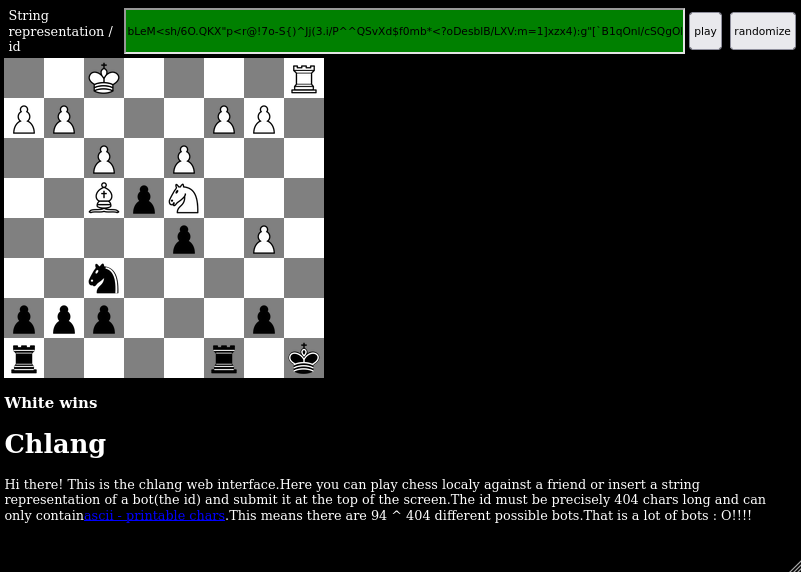
\includegraphics[width=\textwidth]{./images/web.png}
    (bild 1) - skärmdump av hemsidan där boten som spelar vit har vunnit ett parti mot spelaren.

	\newpage
	\section{Disskusion}

    \subsection{Chlang språket}
    Någonting som skulle kunna gjorts annorlunda är valet av att skapa ett eget språk. Det hade nog varit smidigare att använda något existeranda konfigueringsspråk såsom json eller toml eftersom att det är lättare för användarna och dessutom existerar mängder av färdiga verktyg för dessa språk. Min egna parser för chlang blev dessutom rätt dålig, så att använda json eller toml som har färdiga parsers hade förenklat processen och dessutom gjort resultatet snyggare.

    \subsection{Att köra godtyckliga strängar som program}
    Ett av huvudsyftena med detta projekt var att testa hur man skulle kunna implementera någon sorts körning av godtyckliga strängar. De allra flesta språk kräver att du förhåller dig till någon sorts syntax för att det ska gå att köra ditt program. Jag tycker däremot att tanken av att kunna köra en godtycklig sträng är intressant då det, som jag tidigare nämnt, öppnar upp för mer kreativitet då program kan generaras och man kan se det som att man uttforskar en rymd av möjliga program (i detta fall ${94^404}$ stycken), snarare än att skapa ett. Till viss del är projektet inspererat av en youtube video om "random art" av "tsoding" (se källa 1)

	\newpage
	\section{Slutsats}
    För att besvara frågeställningen så går det att representera en schackbot med nästan vilken sträng som helst (se metod/abstract/sammanfattning för att läsa om begränsningarna). Dessa botar varierar mindre en vad jag förväntade mig, både med avsende till vilken nivå de spelar på men även till deras stil. Det verkar som att nästan alla botar spelar dåligt men ändå inte så dåligt att man nästan inte kan förlora. Dessutom verkar nästan alla botar spela väldigt aggresivt. Detta är antagligen för att de är "bra" att ha många rutor att gå till. Så att gå ut tidigt med exempelvis drottningen skapar många möjliga drag vilket ger mycket poäng under evalueringen. 

	\newpage
	\section{Vidare Utveckling}
    Det existerar fortfarande en del buggar i Chlang dom kan fixas. Utöver det så kan man tack vare Eval traiten ganska enkelt uttöka funktionaliteten för Chlang eller använda det som ett bibliotek (en crate i rust) för att skapa andra botar.
    Dessutom kan man antagligen göra mängder med prestanda förbättringar och till exempel implementera parallelisering.
    Websidan behöver dessutom lite mer tilltalanda styling. Men detta var inget fokusområde för projektet.
    Jag skulle också vilja se att man på ett enkelt sätt kan träna botar då det var ett av mina mål. Det utfördes experiment för att testa detta men jag tror dessvärre att man först skulle behöva göra ganska markanta prestandaförbättringar för att det ska vara möjligt. Det utfördes experiment för att testa detta men jag tror dessvärre att man först skulle behöva göra ganska markanta prestandaförbättringar för att det ska vara möjligt. 
	
	\newpage
	\section{Källförteckning}
    \begin{enumerate}
     \item \url{https://www.youtube.com/watch?v=JaG4kdyS_I8&list=PLpM-Dvs8t0VaTz0wuDbwMfilC_JZkZKK5&index=2} 
    \item \url{https://www.chessprogramming.org/}
    \item \url{https://book.leptos.dev/}
    \end{enumerate}

\end{document}

